\documentclass{standalone}
\usepackage{tikz}
\usetikzlibrary{patterns, positioning}
\usepackage[sfdefault]{ClearSans} %% option 'sfdefault' activates Clear Sans as the default text font
\usepackage[T1]{fontenc}

\begin{document}
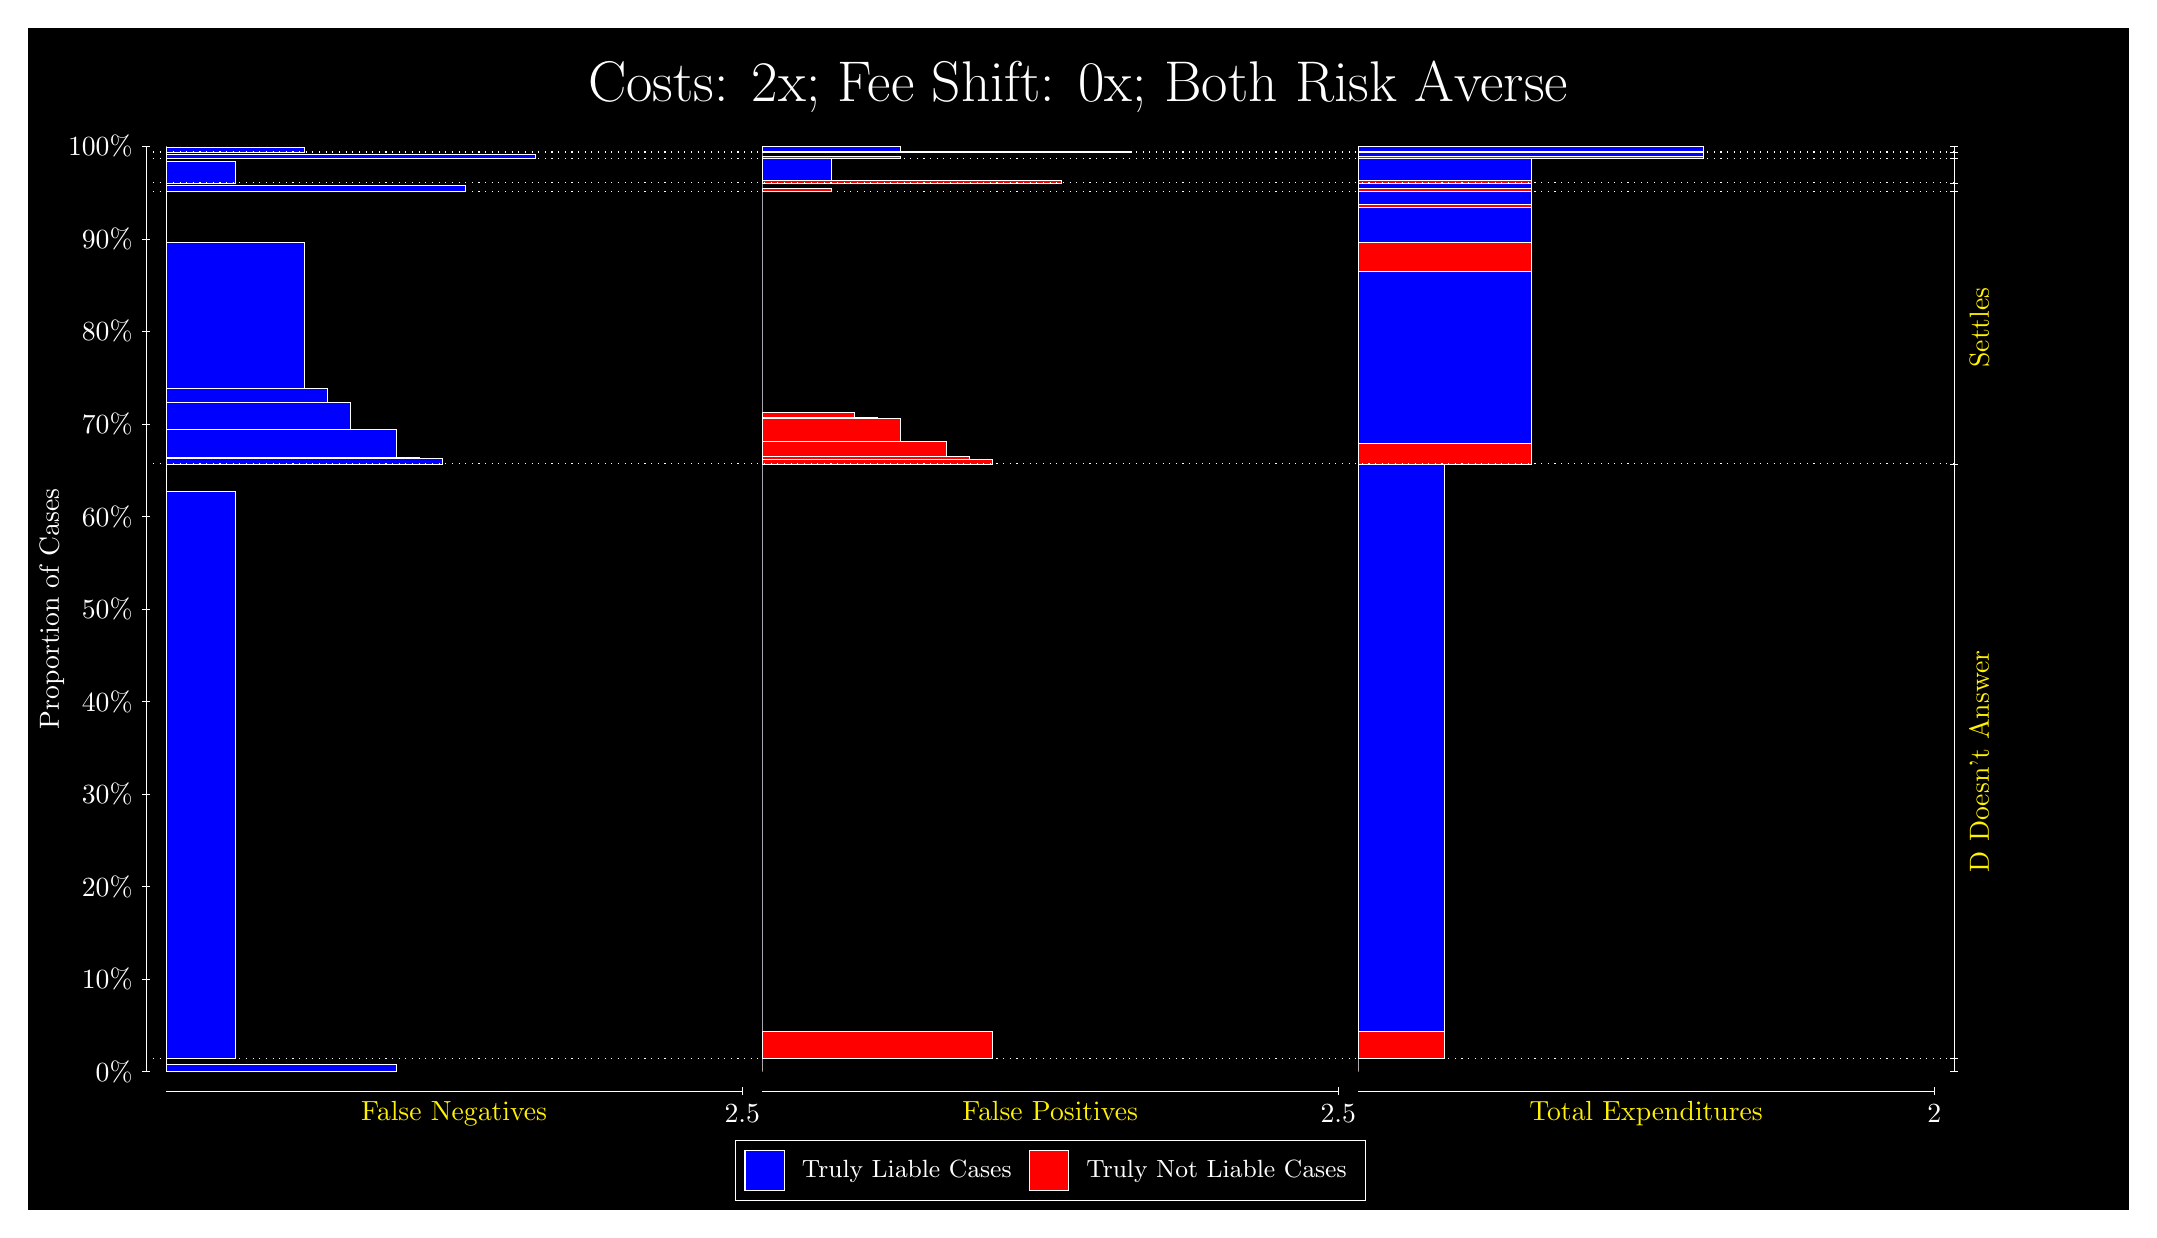
\begin{tikzpicture}
\draw[fill=black] (0,0) rectangle (26.667,15);
\draw[text=white] (0,13.5) rectangle (26.667,15) node[midway] {\huge Costs: 2x; Fee Shift: 0x; Both Risk Averse};
\draw[white, very thin] (1.5,1.75) -- (1.5,13.5);
\node[rotate=90, text=white, anchor=center] at (0.3, 7.625) {Proportion of Cases};
\draw[white, very thin] (1.45,1.75) -- (1.55,1.75);
\node[text=white, anchor=east] at (1.45, 1.75) {0\%};
\draw[white, very thin] (1.45,2.925) -- (1.55,2.925);
\node[text=white, anchor=east] at (1.45, 2.925) {10\%};
\draw[white, very thin] (1.45,4.1) -- (1.55,4.1);
\node[text=white, anchor=east] at (1.45, 4.1) {20\%};
\draw[white, very thin] (1.45,5.275) -- (1.55,5.275);
\node[text=white, anchor=east] at (1.45, 5.275) {30\%};
\draw[white, very thin] (1.45,6.45) -- (1.55,6.45);
\node[text=white, anchor=east] at (1.45, 6.45) {40\%};
\draw[white, very thin] (1.45,7.625) -- (1.55,7.625);
\node[text=white, anchor=east] at (1.45, 7.625) {50\%};
\draw[white, very thin] (1.45,8.8) -- (1.55,8.8);
\node[text=white, anchor=east] at (1.45, 8.8) {60\%};
\draw[white, very thin] (1.45,9.975) -- (1.55,9.975);
\node[text=white, anchor=east] at (1.45, 9.975) {70\%};
\draw[white, very thin] (1.45,11.15) -- (1.55,11.15);
\node[text=white, anchor=east] at (1.45, 11.15) {80\%};
\draw[white, very thin] (1.45,12.325) -- (1.55,12.325);
\node[text=white, anchor=east] at (1.45, 12.325) {90\%};
\draw[white, very thin] (1.45,13.5) -- (1.55,13.5);
\node[text=white, anchor=east] at (1.45, 13.5) {100\%};

\draw[white, very thin] (24.457,1.75) -- (24.457,13.5);
\draw[white, very thin] (24.407,1.75) -- (24.507,1.75);
\node[anchor=west] at (24.407, 1.75) {};
\draw[white, very thin] (24.407,1.9121) -- (24.507,1.9121);
\node[anchor=west] at (24.407, 1.9121) {};
\draw[white, very thin] (24.407,9.4681) -- (24.507,9.4681);
\node[anchor=west] at (24.407, 9.4681) {};
\draw[white, very thin] (24.407,12.93) -- (24.507,12.93);
\node[anchor=west] at (24.407, 12.93) {};
\draw[white, very thin] (24.407,13.036) -- (24.507,13.036);
\node[anchor=west] at (24.407, 13.036) {};
\draw[white, very thin] (24.407,13.344) -- (24.507,13.344);
\node[anchor=west] at (24.407, 13.344) {};
\draw[white, very thin] (24.407,13.428) -- (24.507,13.428);
\node[anchor=west] at (24.407, 13.428) {};
\draw[white, very thin] (24.407,13.5) -- (24.507,13.5);
\node[anchor=west] at (24.407, 13.5) {};

\draw[white, very thin, fill=blue] (1.75,1.75) rectangle (4.6775,1.8393);
\draw[white, very thin, fill=red] (1.75,1.8393) rectangle (1.75,1.9121);
\draw[white, very thin, fill=blue] (1.75,1.9121) rectangle (2.6283,9.1177);
\draw[white, very thin, fill=red] (1.75,9.1177) rectangle (1.75,9.4681);
\draw[white, very thin, fill=blue] (1.75,9.4681) rectangle (5.2631,9.542);
\draw[white, very thin, fill=blue] (1.75,9.542) rectangle (4.9703,9.5467);
\draw[white, very thin, fill=blue] (1.75,9.5467) rectangle (4.6775,9.9108);
\draw[white, very thin, fill=blue] (1.75,9.9108) rectangle (4.092,10.253);
\draw[white, very thin, fill=blue] (1.75,10.253) rectangle (3.7993,10.423);
\draw[white, very thin, fill=blue] (1.75,10.423) rectangle (3.5065,12.276);
\draw[white, very thin, fill=red] (1.75,12.276) rectangle (1.75,12.93);
\draw[white, very thin, fill=blue] (1.75,12.93) rectangle (5.5558,13.004);
\draw[white, very thin, fill=red] (1.75,13.004) rectangle (1.75,13.036);
\draw[white, very thin, fill=blue] (1.75,13.036) rectangle (2.6283,13.309);
\draw[white, very thin, fill=red] (1.75,13.309) rectangle (1.75,13.344);
\draw[white, very thin, fill=blue] (1.75,13.344) rectangle (6.4341,13.404);
\draw[white, very thin, fill=red] (1.75,13.404) rectangle (1.75,13.428);
\draw[white, very thin, fill=blue] (1.75,13.428) rectangle (3.5065,13.493);
\draw[white, very thin, fill=red] (1.75,13.493) rectangle (1.75,13.5);
\draw[white, very thin, fill=red] (9.3189,1.75) rectangle (9.3189,1.8227);
\draw[white, very thin, fill=blue] (9.3189,1.8227) rectangle (9.3189,1.9121);
\draw[white, very thin, fill=red] (9.3189,1.9121) rectangle (12.246,2.2626);
\draw[white, very thin, fill=blue] (9.3189,2.2626) rectangle (9.3189,9.4681);
\draw[white, very thin, fill=red] (9.3189,9.4681) rectangle (12.246,9.5289);
\draw[white, very thin, fill=red] (9.3189,9.5289) rectangle (11.954,9.559);
\draw[white, very thin, fill=red] (9.3189,9.559) rectangle (11.661,9.7527);
\draw[white, very thin, fill=red] (9.3189,9.7527) rectangle (11.075,10.05);
\draw[white, very thin, fill=red] (9.3189,10.05) rectangle (10.783,10.053);
\draw[white, very thin, fill=red] (9.3189,10.053) rectangle (10.49,10.122);
\draw[white, very thin, fill=blue] (9.3189,10.122) rectangle (9.3189,12.93);
\draw[white, very thin, fill=red] (9.3189,12.93) rectangle (10.197,12.962);
\draw[white, very thin, fill=blue] (9.3189,12.962) rectangle (9.3189,13.036);
\draw[white, very thin, fill=red] (9.3189,13.036) rectangle (13.125,13.071);
\draw[white, very thin, fill=blue] (9.3189,13.071) rectangle (10.197,13.344);
\draw[white, very thin, fill=red] (9.3189,13.344) rectangle (11.075,13.368);
\draw[white, very thin, fill=blue] (9.3189,13.368) rectangle (9.3189,13.428);
\draw[white, very thin, fill=red] (9.3189,13.428) rectangle (14.003,13.435);
\draw[white, very thin, fill=blue] (9.3189,13.435) rectangle (11.075,13.5);
\draw[white, very thin, fill=red] (16.888,1.75) rectangle (16.888,1.8227);
\draw[white, very thin, fill=blue] (16.888,1.8227) rectangle (16.888,1.9121);
\draw[white, very thin, fill=red] (16.888,1.9121) rectangle (17.986,2.2626);
\draw[white, very thin, fill=blue] (16.888,2.2626) rectangle (17.986,9.4681);
\draw[white, very thin, fill=red] (16.888,9.4681) rectangle (19.083,9.7226);
\draw[white, very thin, fill=blue] (16.888,9.7226) rectangle (19.083,11.918);
\draw[white, very thin, fill=red] (16.888,11.918) rectangle (19.083,12.287);
\draw[white, very thin, fill=blue] (16.888,12.287) rectangle (19.083,12.73);
\draw[white, very thin, fill=red] (16.888,12.73) rectangle (19.083,12.76);
\draw[white, very thin, fill=blue] (16.888,12.76) rectangle (19.083,12.93);
\draw[white, very thin, fill=red] (16.888,12.93) rectangle (19.083,12.962);
\draw[white, very thin, fill=blue] (16.888,12.962) rectangle (19.083,13.036);
\draw[white, very thin, fill=red] (16.888,13.036) rectangle (19.083,13.071);
\draw[white, very thin, fill=blue] (16.888,13.071) rectangle (19.083,13.344);
\draw[white, very thin, fill=red] (16.888,13.344) rectangle (21.279,13.368);
\draw[white, very thin, fill=blue] (16.888,13.368) rectangle (21.279,13.428);
\draw[white, very thin, fill=red] (16.888,13.428) rectangle (21.279,13.435);
\draw[white, very thin, fill=blue] (16.888,13.435) rectangle (21.279,13.5);
\draw[white, dotted] (1.5,1.9121) -- (24.457,1.9121);
\draw[white, dotted] (1.5,9.4681) -- (24.457,9.4681);
\draw[white, dotted] (1.5,12.93) -- (24.457,12.93);
\draw[white, dotted] (1.5,13.036) -- (24.457,13.036);
\draw[white, dotted] (1.5,13.344) -- (24.457,13.344);
\draw[white, dotted] (1.5,13.428) -- (24.457,13.428);
\draw[white, very thin] (1.75,1.5) -- (9.0689,1.5);
\node[text=yellow, anchor=north] at (5.4094, 1.5) {False Negatives};
\draw[white, very thin] (9.0689,1.45) -- (9.0689,1.55);
\node[text=white, anchor=north] at (9.0689, 1.45) {2.5};

\draw[white, very thin] (9.3189,1.5) -- (16.638,1.5);
\node[text=yellow, anchor=north] at (12.978, 1.5) {False Positives};
\draw[white, very thin] (16.638,1.45) -- (16.638,1.55);
\node[text=white, anchor=north] at (16.638, 1.45) {2.5};

\draw[white, very thin] (16.888,1.5) -- (24.207,1.5);
\node[text=yellow, anchor=north] at (20.547, 1.5) {Total Expenditures};
\draw[white, very thin] (24.207,1.45) -- (24.207,1.55);
\node[text=white, anchor=north] at (24.207, 1.45) {2};


\node[text=yellow, centered, rotate=90] at (24.777, 5.6901) {D Doesn't Answer};
\node[text=yellow, centered, rotate=90] at (24.777, 11.199) {Settles};





\draw (12.978300999999998,1.5) node[draw=none] (baseCoordinate) {};
\begin{scope}[align=center]
        \matrix[scale=0.5, draw=white, below=0.5cm of baseCoordinate, nodes={draw}, column sep=0.1cm]{
            \node[rectangle, draw, minimum width=0.5cm, minimum height=0.5cm, fill=blue] {}; &
            \node[draw=none, font=\small, text=white] (B) {Truly Liable Cases}; &
            \node[rectangle, draw, minimum width=0.5cm, minimum height=0.5cm, fill=red] {}; &
            \node[draw=none, font=\small, text=white] (B) {Truly Not Liable Cases}; \\
            };
\end{scope}

\end{tikzpicture}
\end{document}